\chapter{Aplikacja Twitter Analyser}
\qquad Narzędziem stworzonym w ramach pracy dyplomowej jest aplikacja nazwana \textit{Twitter Analyser}. Rozwiązanie to zostało zaimplementowane z użyciem narzędzi wymienionych w poprzednim rozdziale. Jest to webowa aplikacja działająca lokalnie, która po odpowiedniej konfiguracji, może zostać zainstalowana na komputerze. 

System ten posiada dwie główne funkcjonalności:

\begin{enumerate}
	\item Przetwarzanie interesujących danych ze strumienia udostępnionego przez portal społecznościowy Twitter i zapis ich do bazy danych;
	\item Analizowanie zapisanych danych pod względem wydźwięku zamieszczanych opinii oraz powiązań między użytkownikami.
\end{enumerate}

Główny ekran narzędzia, widoczny na rysunku 6.1, prezentuje podstawowe informacje o aplikacji oraz jej podstronach, a także umożliwia przejście na nie.

\begin{figure}[h] % h means here
	\centering
	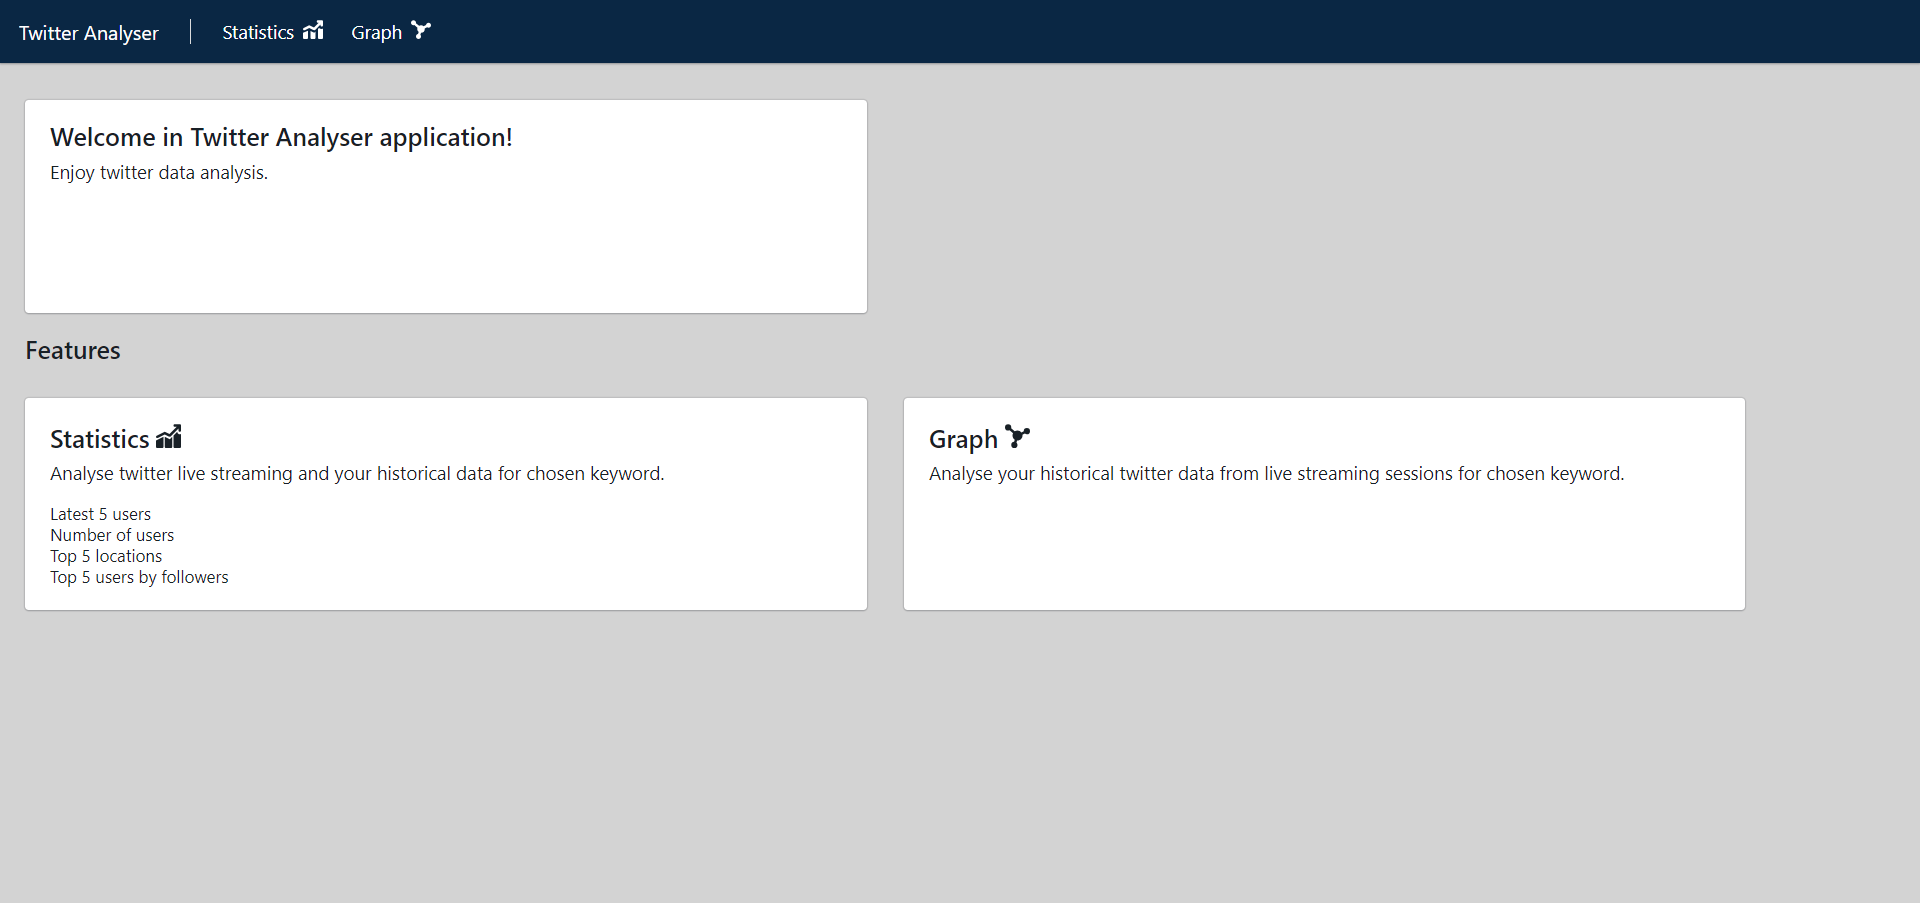
\includegraphics[width=1.0\linewidth]{img/twitter_analyser_1}
	\caption{Ekran startowy aplikacji \textit{Twitter Analyser} [materiały własne].}
\end{figure}

\textcolor{white}{.}

\textbf{Strona Statistics}

Pierwsza ze wspomnianych funkcjonalności jest dostępna na stronie \textit{Statistics}, której zrzut ekranu jest widoczny na rysunku 6.2.. Interfejs użytkownika na tej stronie prezentuje podstawowe statystyki z przeprowadzanej właśnie sesji analizy danych. Są to:

\begin{itemize}
	\item[--] nazwy ostatnich pięciu użytkowników,
	\item[--] liczba wszystkich użytkowników,
	\item[--] nazwy pięciu najczęściej pojawiających się lokalizacji,
	\item[--] nazwy pięciu użytkowników z największą liczbą osób ślędzących ich profil tzw. followersów,
	\item[--] treść pięciu ostatnich wiadomości tzw. tweetów,
	\item[--] treść pięciu ostatnich wiadomości przekazywanych dalej tzw. retweetów.
\end{itemize}

\begin{figure}[h] % h means here
	\centering
	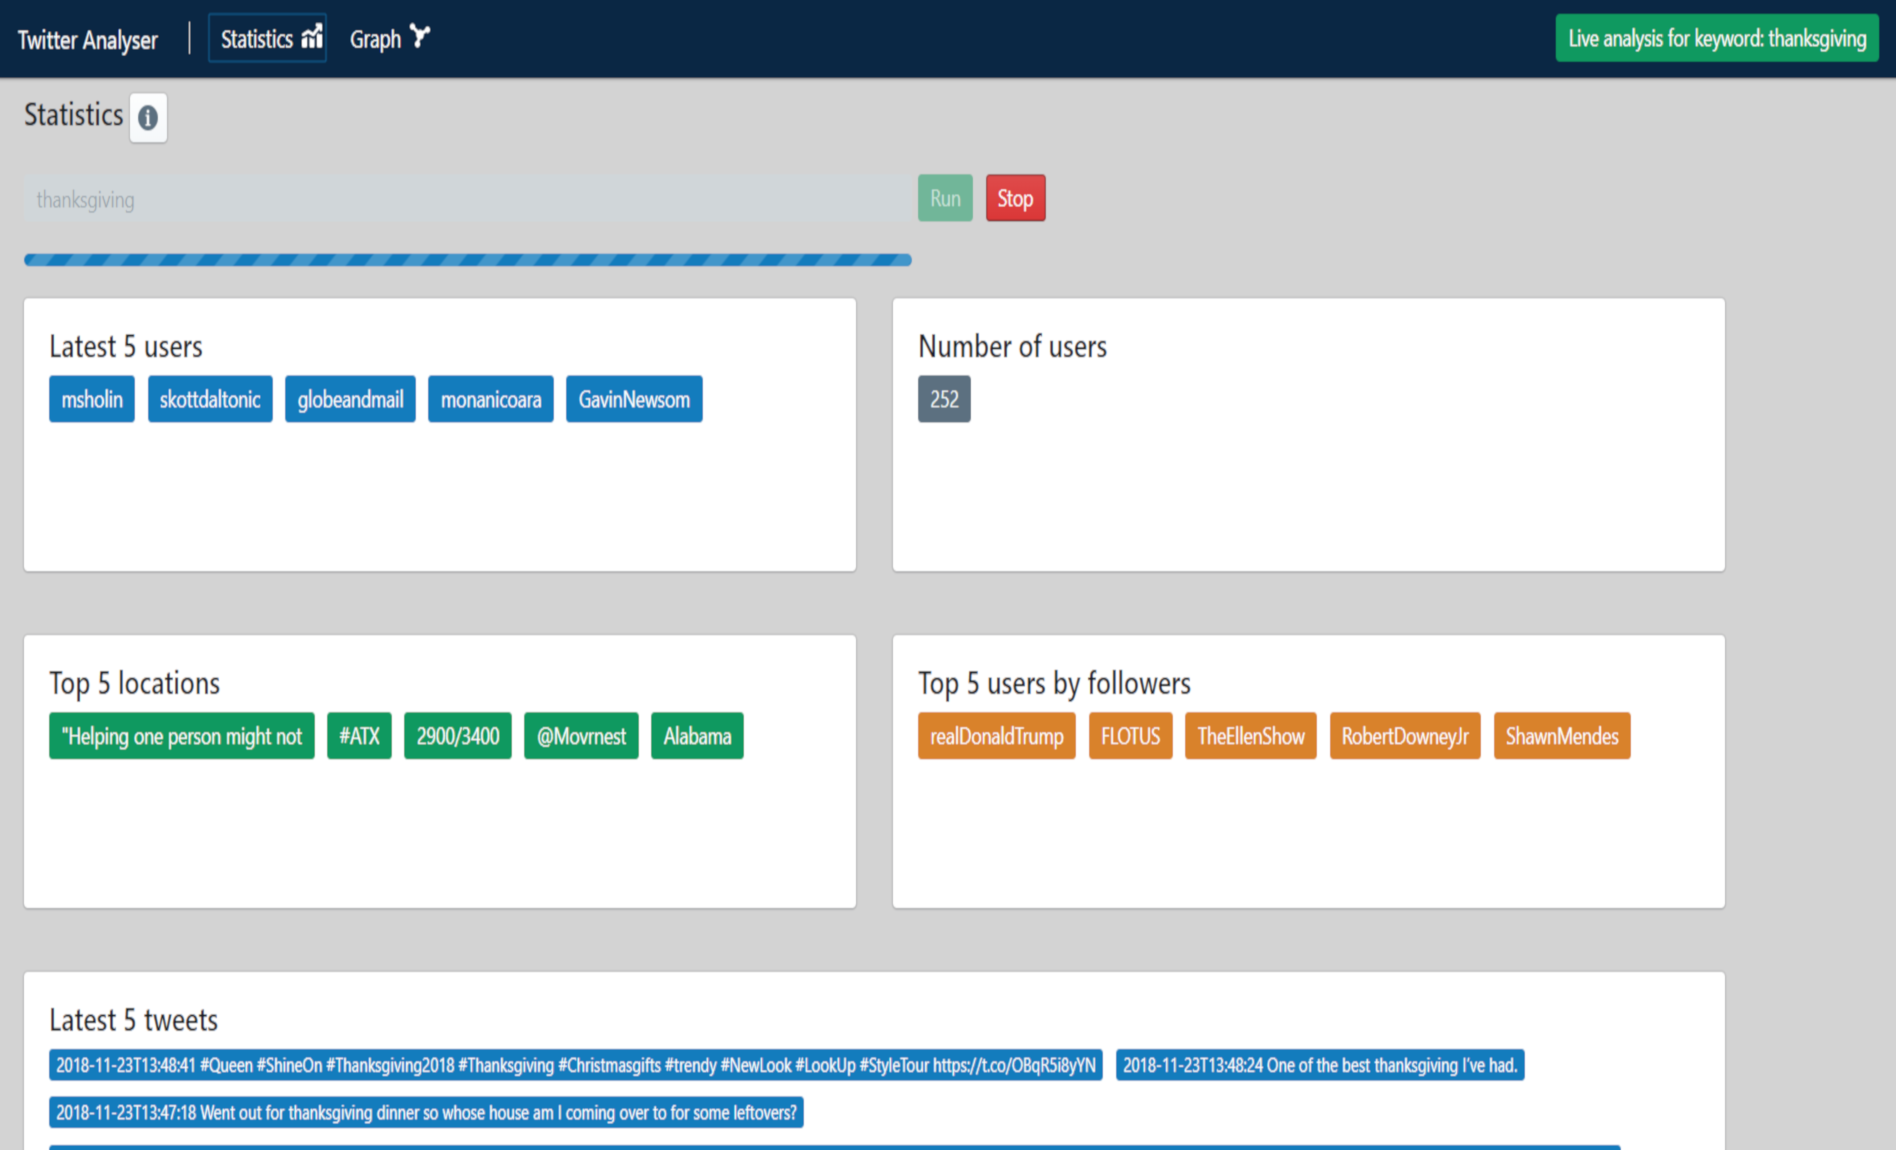
\includegraphics[width=1.0\linewidth]{img/twitter_analyser_thanks_giving_2}
	\caption{Interfejs graficzny strony \textit{Statistics} podczas przetwarzania postów zawierających w treści wyrażenie \textit{thanksgiving} związane ze Świętem Dziękczynienia obchodzonym w Stanach Zjednoczonych [materiały własne].}
\end{figure}

Rozpoczęcie przetwarzania danych następuje w momencie kiedy po wpisaniu przez użytkownika interesującego go słowa kluczowego uruchomi on wspomniany proces przyciskiem Run. Konsekwencją tego jest skonfigurowanie oraz uruchomienie Apache Spark podłączonego do strumienia danych Twitter Streaming API. Aby uzyskać dostęp do tej porcji danych należy zarejestrować wcześniej aplikację i dostać od serwisu Twitter poświadczenia to umożliwiające. Są to unikatowe: \textit{consumer key}, \textit{consumer secret}, \textit{access token} i \textit{access token secret}. Fragment konfiguracji Apache Spark zamieszczono na rysunku 6.3..

\begin{figure}[h] % h means here
	\centering
	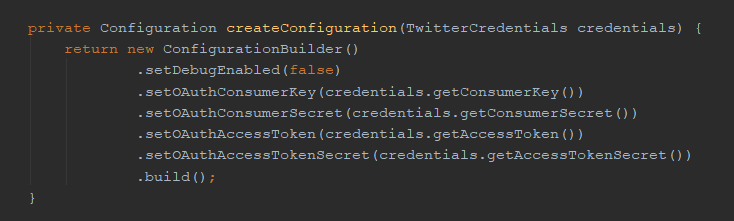
\includegraphics[width=0.8\linewidth]{img/twitter_analyser_apache_spark_configuration}
	\caption{Fragment konfiguracji narzędzia \textit{Apache Spark} [materiały własne].}
\end{figure}

Na podstawie przeprowadzonych testów stwierdzono, że czas trwania pojedynczego okna czasowego powinien wynieść 10 sekund. Jest to czas, który pozwala przetworzyć odebrane wiadomości i nie powoduje opóźnień.

Mechanizm przetwarzania danych, którego kod jest widoczny na rysunkach 6.4 oraz 6.5, polega w pierwszej kolejności na sprawdzeniu czy były już przeprowadzane sesje analizy danych z użyciem wybranego słowa kluczowego. Jeśli tak było to wyniki obecnie uruchomionej sesji będą połączone z wynikami z historycznych danych powiązanych z zapisaną encją Keyword. Kolejnym krokiem jest filtracja strumienia danych pod kątem zawartości słowa kluczowego w treści postów. Wielkość liter słowa kluczowego wybranego przez użytkownika aplikacji Twitter Analyser nie ma znaczenia. Potem przefiltrowany strumień jest zamieniany na strumień par \textit{<User, Status>}, gdzie \textit{User} i \textit{Status} odpowiadają klasom implementującym interfejsy opisane w rozdziale 2.. Końcowym etapem jest zapis informacji o użytkowniku oraz jego wiadomości na podstawie wspomnianego strumienia. Jeśli użytkownik pojawił się wcześniej podczas uruchamianych sesji to właśnie przetwarzana wiadomość zostanie dodana do wcześniejszych informacji o nim zapisanej w encji TwitterUser. Status umożliwia m.in. odczytanie informacji czy wiadomość jest wiadomością własną użytkownika czyli tzw. tweet czy podaną dalej tzw. retweet. Stąd biorą się dwa typy relacji występujące w obowiązującym w tworzonej aplikacji modelu danych. Przygotowanie relacji między węzłami wykorzystuje informacje o słowie kluczowym, użytkowniku którego post jest obecnie przetwarzany oraz jego statusie. Metoda odpowiedzialna za przygotowanie relacji typu RetweetedToRelation posługuje się rekurencją, czyli wywoływaniem samej siebie, z powodu możliwych przypadków przekazywania dalej przekazanej już przez innego użytkownika wiadomości.

\begin{figure}[h] % h means here
	\centering
	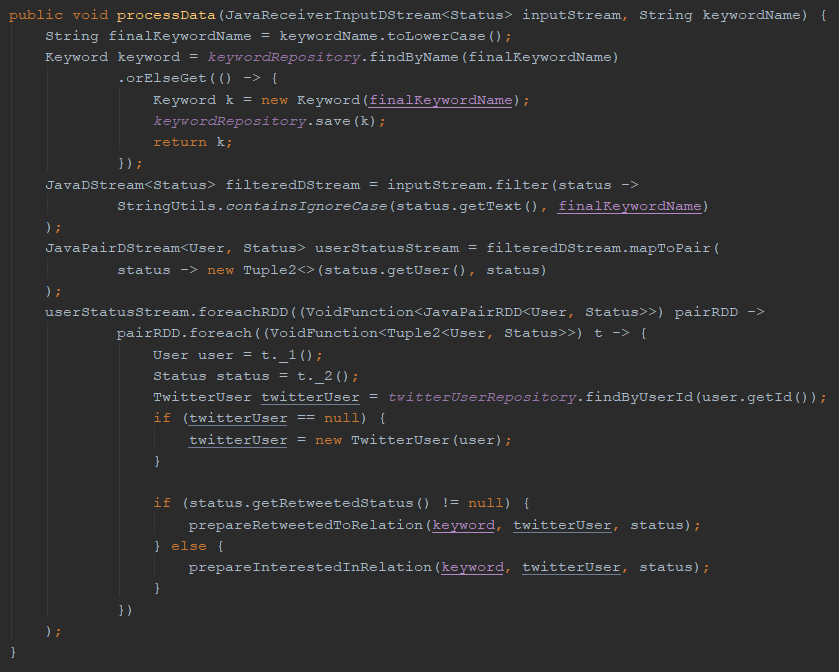
\includegraphics[width=1.0\linewidth]{img/twitter_analyser_process_data}
	\caption{Przetwarzanie danych ze strumienia udostępnianego przez serwis społecznościowy \textit{Twitter} [materiały własne].}
\end{figure}

Wspomniane typy relacji posiadają odpowiadające im encje InterestedInRelation oraz RetweetedToRelation widoczne na rysunkach 6.6 i 6.7.. Odpowiadają one połączeniom między węzłami. W przypadku pierwszej z nich jest to powiązanie węzłów typu TwitterUser i Keyword. Jest ono skierowane ku temu drugiemu. Drugi typ relacji odpowiada połączeniu pomiędzy węzłami typu TwitterUser i jest skierowane ku użytkownikowi, którego wiadomość została przesłana dalej. Graficzną reprezentację modelu danych zaprezentowano na rysunku 6.10..

\begin{figure}[h] % h means here
	\centering
	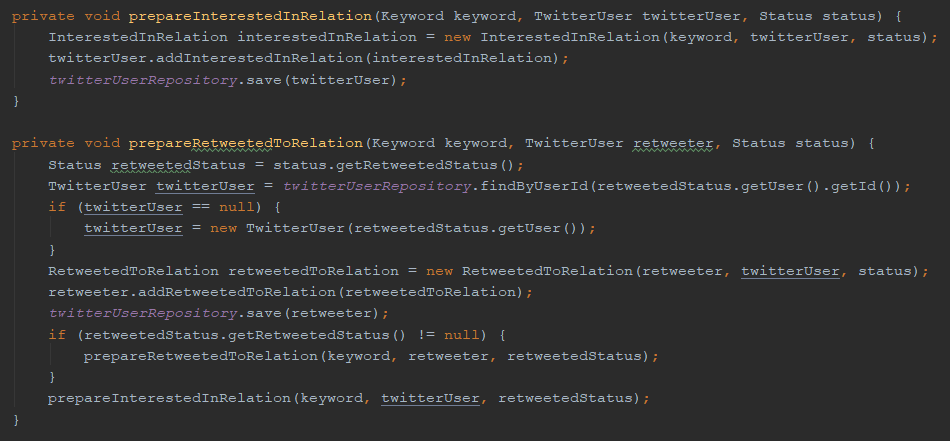
\includegraphics[width=1.0\linewidth]{img/twitter_analyser_process_data_2}
	\caption{Przygotowywanie i zapis relacji pomiędzy użytkownikami [materiały własne].}
\end{figure}

\begin{figure}[h] % h means here
	\centering
	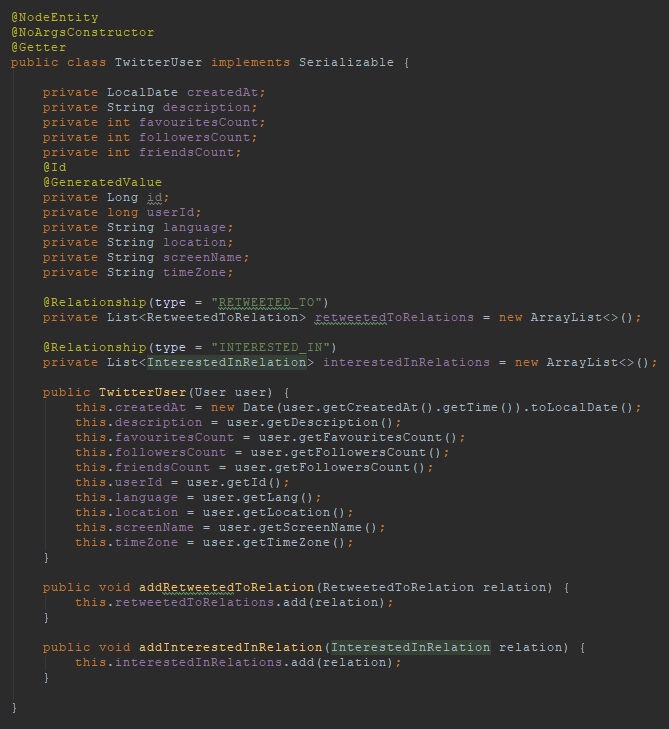
\includegraphics[width=1.0\linewidth]{img/twitter_analyser_twitter_user}
	\caption{Kod encji \textit{TwitterUser} [materiały własne].}
\end{figure}

\begin{figure}[h] % h means here
	\centering
	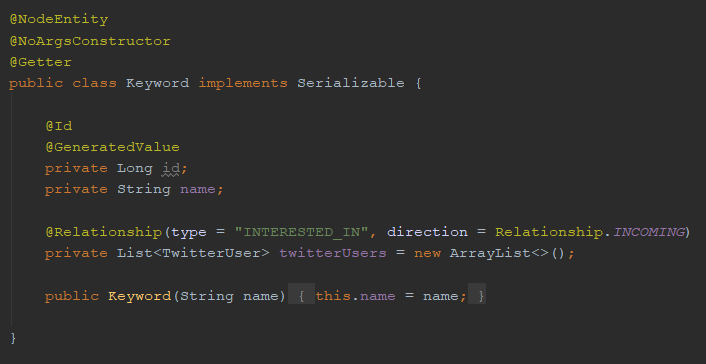
\includegraphics[width=1.0\linewidth]{img/twitter_analyser_keyword}
	\caption{Kod encji \textit{Keyword} [materiały własne].}
\end{figure}

\begin{figure}[h] % h means here
	\centering
	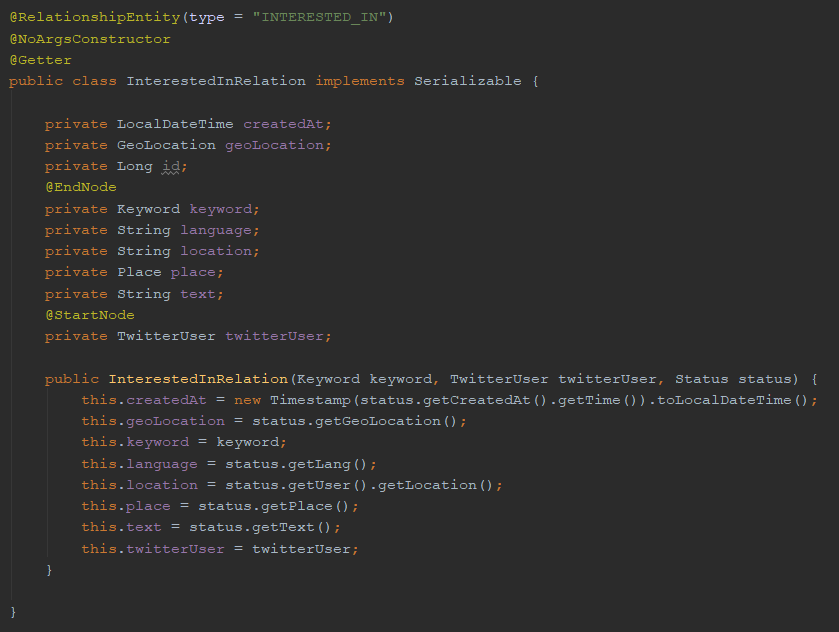
\includegraphics[width=1.0\linewidth]{img/twitter_analyser_interested_in_relation}
	\caption{Kod encji relacji \textit{InterestedInRelation} [materiały własne].}
\end{figure}

\begin{figure}[h] % h means here
	\centering
	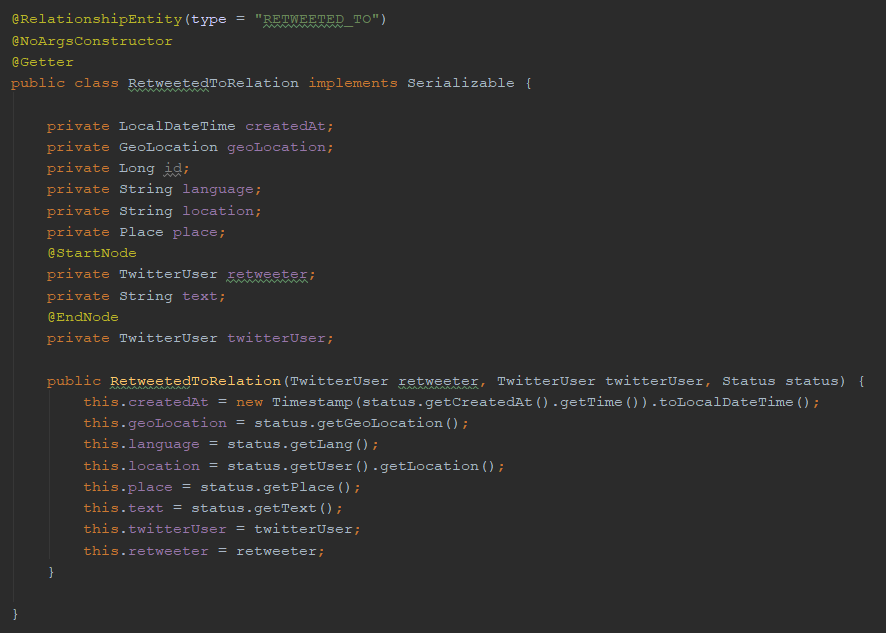
\includegraphics[width=1.0\linewidth]{img/twitter_analyser_retweeted_to_relation}
	\caption{Kod encji relacji \textit{RetweetedToRelation} [materiały własne].}
\end{figure}

\begin{figure}[h] % h means here
	\centering
	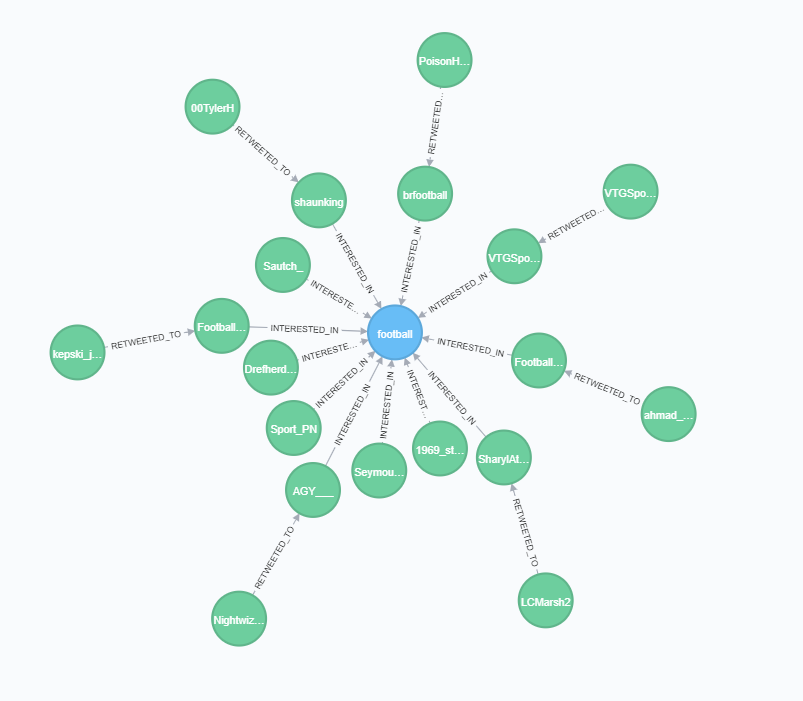
\includegraphics[width=1.0\linewidth]{img/big_data_neo4j}
	\caption{Graficzna reprezentacja modelu danych. Niebieski węzeł jest typu \textit{Keyword}, a pozostałe zielone typu \textit{TwitterUser}. Pomiędzy węzłami występują relacje typu \textit{InterestedInRelation} oraz \textit{RetweetedToRelation} [materiały własne].}
\end{figure}

Informacje o przetwarzanych wiadomościach i użytkownikach pobierane są z grafowej bazy danych, a następnie przesyłane z serwera do przeglądarki internetowej co 10 s za pomocą dwukierunkowego kanału komunikacji o nazwie \textit{WebSocket}, który wykorzystuje protokół TCP [25]. Rozpoczęcie przesyłania danych jest inicjowane przez przeglądarkę internetową. Następnie pomiędzy klientem a serwerem następuje nawiązanie komunikacji. Serwer wysyła statystyki z przeprowadzanej właśnie sesji analizy danych co ustalony czas bez ciągłego wymuszania tej akcji ze strony klienta. Konfigurację po stronie serwera aplikacyjnego zaprezentowano na rysunkach 6.6 oraz 6.7..

\begin{figure}[h] % h means here
	\centering
	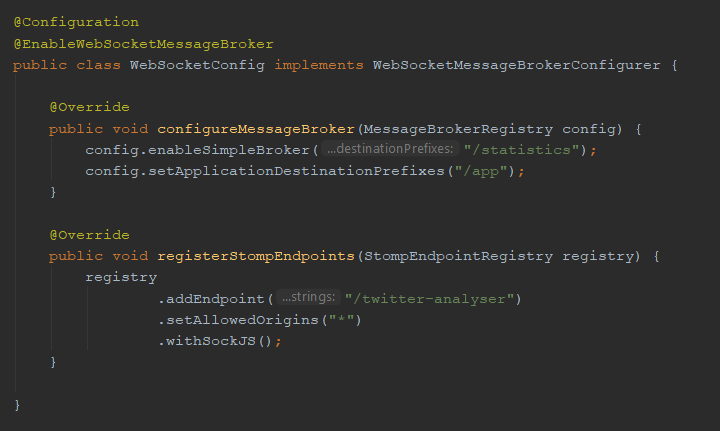
\includegraphics[width=1.0\linewidth]{img/twitter_analyser_websocket_configuration_2}
	\caption{Konfiguracja dwukierunkowego kanału komunikacji \textit{WebSocket} [materiały własne].}
\end{figure}

\begin{figure}[h] % h means here
	\centering
	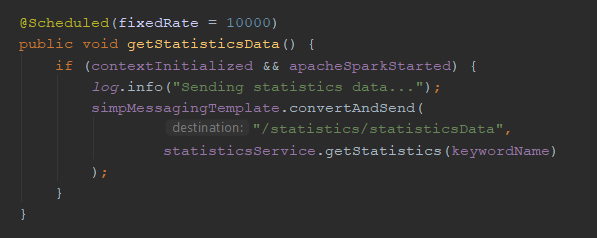
\includegraphics[width=1.0\linewidth]{img/twitter_analyser_websocket_configuration_1}
	\caption{Konfiguracja dwukierunkowego kanału komunikacji \textit{WebSocket} [materiały własne].}
\end{figure}

\textbf{Strona Graph}

Druga z głównych funkcjonalności programu czyli analiza zapisanych danych pod względem wydźwięku zamieszczanych opinii oraz powiązań między użytkownikami jest dostępna na stronie \textit{Graph}, której zrzut ekranu widoczny jest na rysunku 6.13.. Interfejs użytkownika na tej stronie prezentuje szczegółowy wykres węzłów połączonych relacjami. 

Rozpoczęcie analizowania danych następuje w momencie wyboru słowa kluczowego jakie zostało podane podczas sesji na stronie Statistics. Po kliknięciu przycisku Search następuje przesłanie polecenia do serwera o wyszukanie w bazie danych wszystkich danych będących w korelacji z tym słowem kluczowym. Kolejnym krokiem jest przetworzenie danych i zapisanie ich do modelu, z którego będzie mogła skorzystać przeglądarka. Tak przygotowane dane są przesyłane do klienta, a następnie wyświetlone w postaci wykresu węzłów powiązanych relacjami. Kolor każdego z węzłów jest określany na podstawie sentymentu obliczonego z postów, które zamieścił użytkownik. Sentyment bardzo pozytywny jest określany kolorem ciemnozielonym, pozytywny zielonym, neutralny szarym, negatywny pomarańczowym, a bardzo negatywny czerwonym. Jeśli przynajmniej jeden z postów użytkownika nie jest napisany w języku angielskim to dla takiego profilu nie jest obliczany wydźwięk wypowiedzi i kolor węzła jest biały. Ponad wykresem widnieją statystyki pokazujące ilu użytkowników jest dostępnych w bieżącej analizie oraz ich podział procentowy i liczbowy ze względu na sentyment. Istnieje także możliwość uzyskania szczegółowych informacji o użytkowniku poprzez kliknięcie w węzeł na wykresie. Zrzut ekranu okienka typu pop-up zawierającego te dane zaprezentowano na rysunku 6.14.. Informacje dotyczące relacji łączącej węzły są dostępne poprzez kliknięcie w nie. Zrzut ekranu okienka znajduje się na rysunku 6.15.. W obu przypadkach dane są pobierane z bazy dopiero w momencie kliknięcia. Optymalizacja ta została wykonana aby nie przesyłać niepotrzebnych informacji i nie obciążać mechanizmy odpowiadające za wyświetlenie wykresu.

Mechanizm przetwarzania danych, którego część kodu jest widoczna na rysunku 6.16., polega w pierwszej kolejności na pobraniu z grafowej bazy informacji powiązanych z wybranym słowem kluczowym. W następnym kroku kolekcja obiektów TwitterUser jest mapowana na kolekcję obiektów typu Node. Podczas wykonywania operacji mapowania następuje wspomniane sprawdzenie czy user napisał wszystkie posty w języku angielskim. Taka informacja jest dostępna dla każdego posta podczas przetwarzania danych ze strumienia danych serwisu Twitter i wówczas zapisywana do bazy. Sentyment każdego z postów jest obliczany niezależnie, a następnie aplikacja oblicza średnią arytmetyczną i przyporządkowuje wydźwięk z pięciostopniowej skali.

Napisany algorytm obliczania sentymentu rozpoczyna swoje działanie od usunięcia z treści posta słów z prefixem '@' oraz adresów internetowych, ponieważ w innym wypadku zaburzałoby to działanie tego algorytmu. Tak przygotowany tweet przekazywany jest do mechanizmów biblioteki Stanford NLP, która dzieli go na zdania. Dla każdego ze zdań obliczany jest sentyment z wykorzystaniem wytrenowej sieci neuronowej dostarczanej przez tą bibliotekę. Wydźwięk tekstu obliczany jest jako średnia arytmetyczna sentymentu każdego ze zdań.

\begin{figure}[h] % h means here
	\centering
	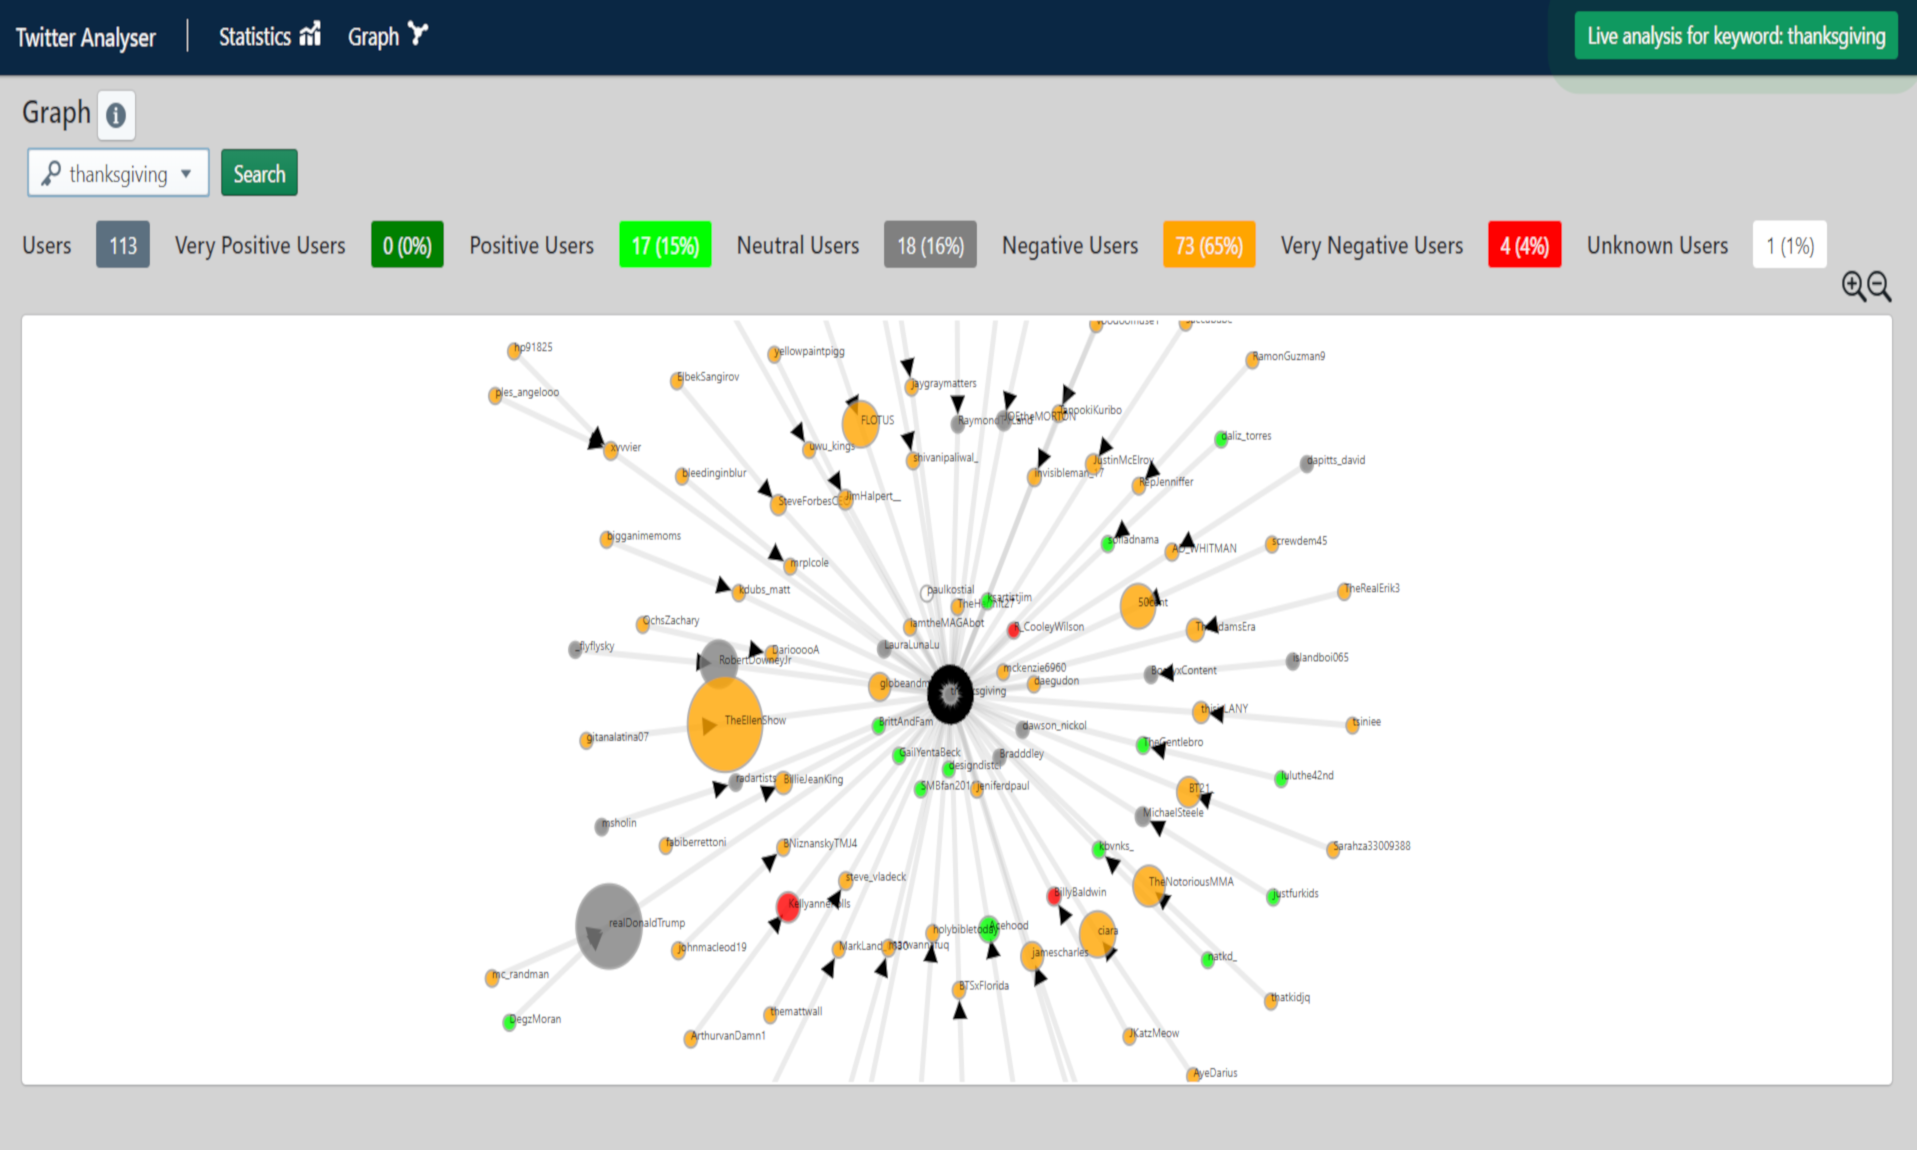
\includegraphics[width=1.0\linewidth]{img/twitter_analyser_thanks_giving_1}
	\caption{Interfejs graficzny strony \textit{Graph} podczas analizy danych związanych ze Świętem Dziękczynienia obchodzonym w Stanach Zjednoczonych [materiały własne].}
\end{figure}

\begin{figure}[h] % h means here
	\centering
	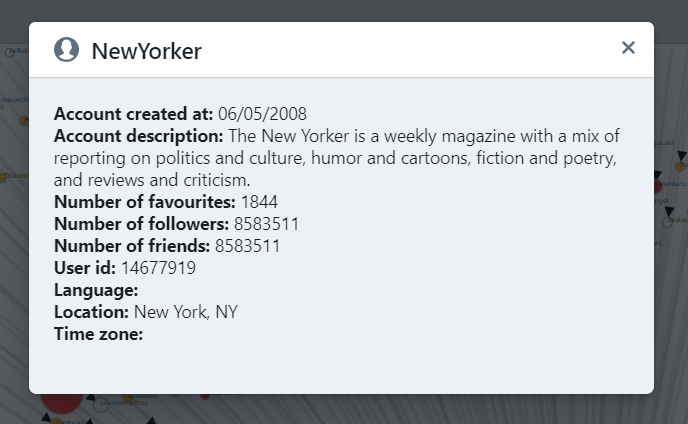
\includegraphics[width=0.6\linewidth]{img/twitter_analyser_user_profile}
	\caption{Okienko typu pop-up służące do wyświetlenia informacji o użytkowniku [materiały własne].}
\end{figure}

\begin{figure}[h] % h means here
	\centering
	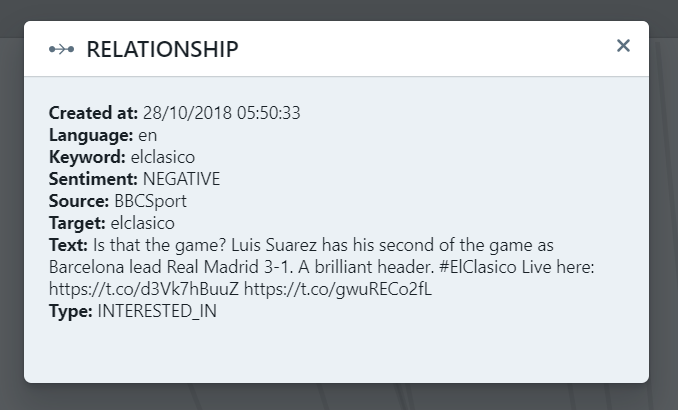
\includegraphics[width=0.6\linewidth]{img/twitter_analyser_relationship}
	\caption{Okienko typu pop-up służące do wyświetlenia informacji o relacji łączącej węzły [materiały własne].}
\end{figure}

\begin{figure}[h] % h means here
	\centering
	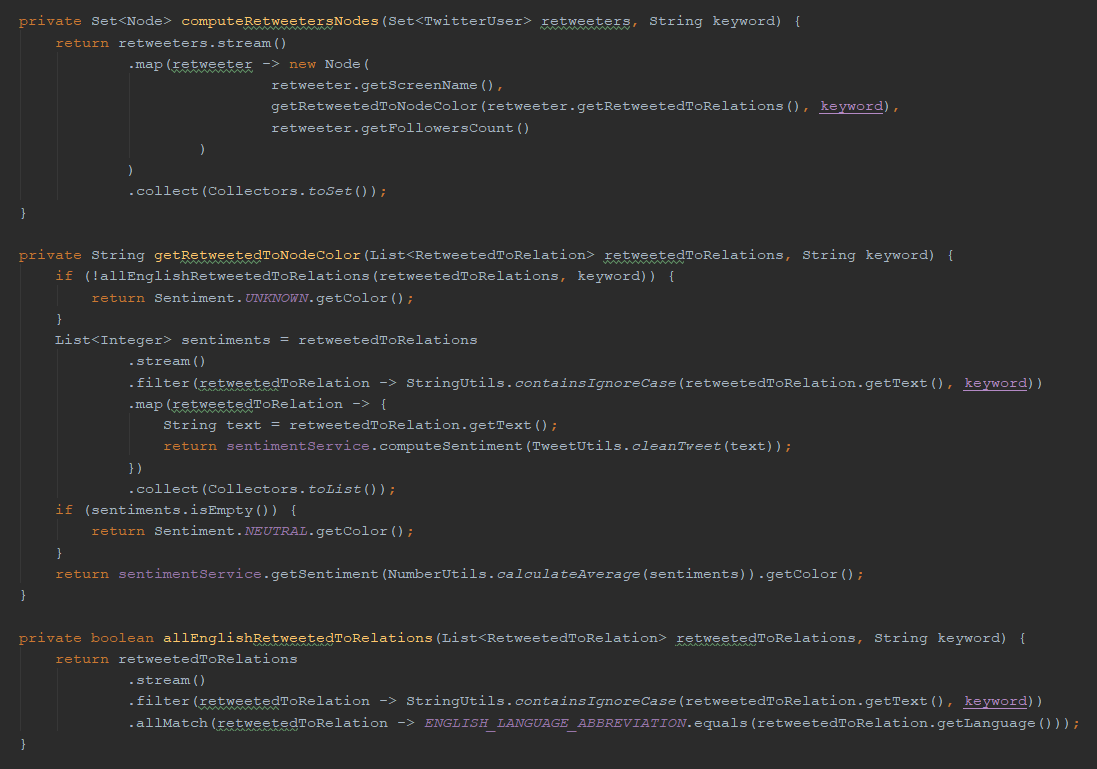
\includegraphics[width=1.0\linewidth]{img/twitter_analyser_compute_retweeters_nodes}
	\caption{Przygotowanie danych dotyczących użytkowników publikujących wiadomości innych autorów. [materiały własne]}
\end{figure}

\textbf{Ogólne informacje o aplikacji}

Użytkownik może korzystać ze stron aplikacji w niezależny sposób. Podczas uruchomienia przetwarzania danych na stronie Statistics można korzystać ze strony Graph i na odwrót. Umożliwia to m.in. analizowanie zgromadzonych danych na stronie Graph tuż po ich zapisaniu przez część serwera powiązaną ze stroną Statistics.

Zarówno strona Graph jak i Statistics posiadają pomoc, która ułatwia korzystanie z aplikacji nowym użytkownikom. Zrzut ekranu okienka typu pop-up z opisanym korzystaniem z funkcjonalności na stronie Graph zamieszczono na rysunku 6.17..

Aplikacja korzysta z ogólnodostępnych danych serwisu Twitter. Pozwala zaobserwować korelacje między użytkownikami oraz wydźwięk ich wypowiedzi, które to informacje byłyby trudne do przeanalizowania przez człowieka z powodu dużego wolumenu danych, ich złożoności oraz zmienności w czasie.

Odporność na błędy aplikacji Twitter Analyser zależy w głównej mierze od mechanizmów narzędzi z których ona korzysta. Nawet nieprawidłowe zachowanie jednego z nich, które może doprowadzić do zatrzymania działania aplikacji, nie wpłynie jednak na już przetworzone i zapisane dane. Ponadto strona Graph może działać bez połączenia z internetem.

System napisany na potrzeby tej pracy dyplomowej spełnia wszystkie wymagania funkcjonalne i niefunkcjonalne postawione w rozdziale 4..

\begin{figure}[h] % h means here
	\centering
	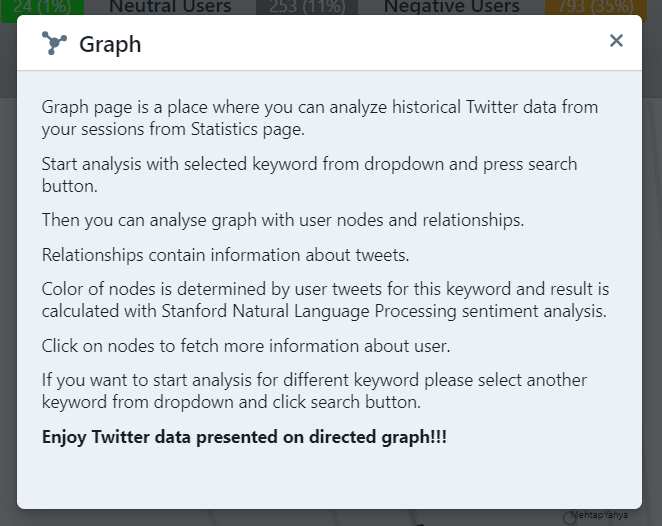
\includegraphics[width=0.6\linewidth]{img/twitter_analyser_help}
	\caption{Okienko typu pop-up służące do wyświetlenia krótkiej informacji o funkcjonalności strony \textit{Graph} [materiały własne].}
\end{figure}

\begin{figure}[h] % h means here
	\centering
	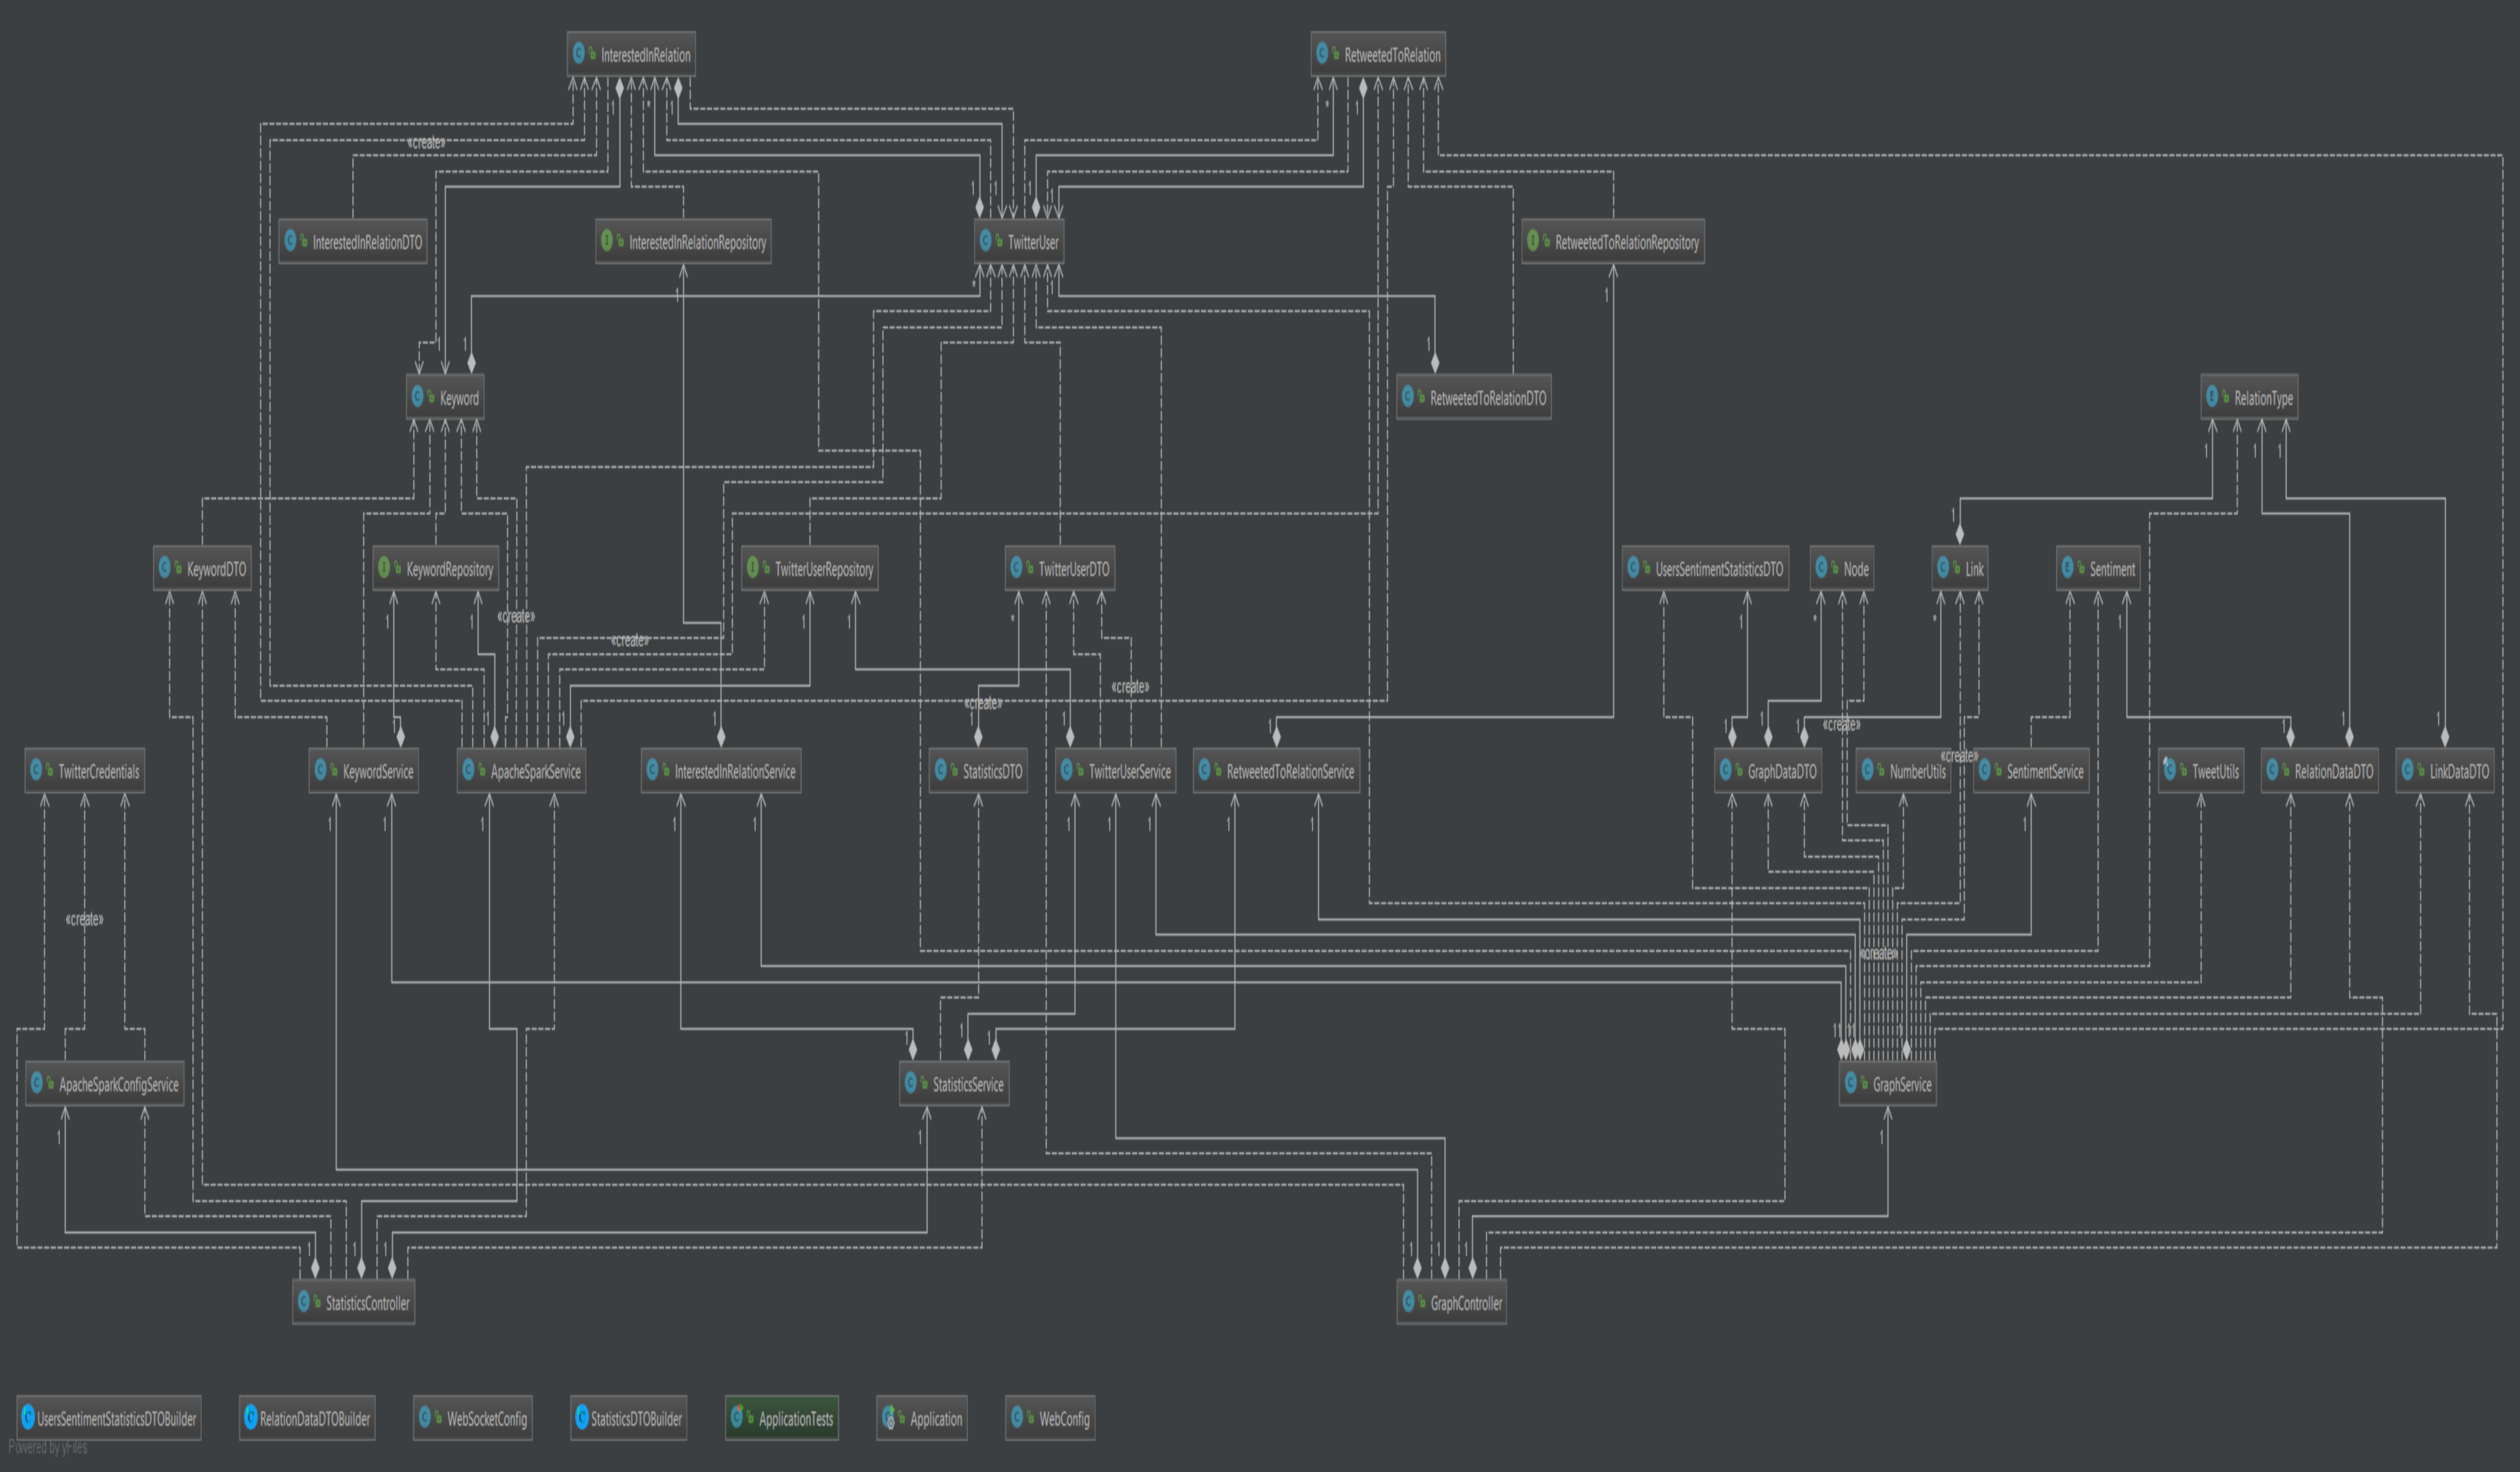
\includegraphics[width=1.5\linewidth, angle=90]{img/twitter_analyser_class_diagram}
	\caption{Diagram klas aplikacji \textit{Twitter Analyser} [materiały własne].}
\end{figure}


